\documentclass[conference]{IEEEtran}
\usepackage{graphicx}
\usepackage{listings}
\usepackage{hyperref}

\hypersetup{
    colorlinks=true,
    linkcolor=blue,
    filecolor=magenta,      
    urlcolor=cyan,
}

\begin{document}

\title{AURO REPORT}
\author{\IEEEauthorblockN{Examination Number: [Your Examination Number Here]}
\IEEEauthorblockA{\textit{Module Code: COM00052H}}
}

\maketitle

\section{Assessment Introduction}
For this assessment, we've been tasked with programming autonomous mobile robots, specifically the TurtleBot3 Waffle Pi, to navigate through a simulated environment with obstacles, and retrieve items scattered around before returning them to the home zone.

\section{Design}
\subsection{System Overview}
% Describe the high-level design of your system. Justify your design choices.
In the design of my autonomous robot, I implemented a modular approach with the TurtleBot3, using the ROS2 framework. At the heart of the design is a finite state machine (FSM), which contains the robot's states - FORWARD, TURNING, COLLECTING, and RETURNING. I chose this FSM for its ability to provide structured yet flexible control, which is essential for navigation and adapting to dynamic task requirements. The keys to perception were the LiDAR and camera sensors, which are essential for effective operation. Their integration within ROS2 is indispensable for the task.

\begin{figure}[htbp]
\centerline{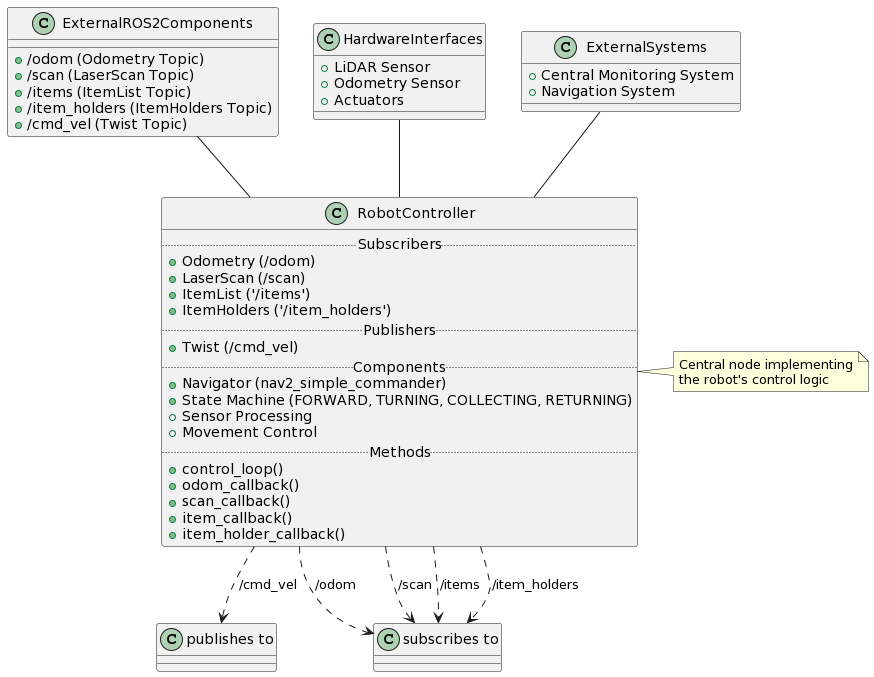
\includegraphics[width=\linewidth]{high-level system diagram.png}}
\caption{High-Level System Design}
\label{fig:systemdesign}
\end{figure}

\subsection{Component Interaction}
%Discuss how the components of your system interact. Refer to Fig.~\ref{fig:systemdesign}.
As shown in Fig.~\ref{fig:systemdesign}, the robot controller subscribes to several essential topics for efficient operation:

\begin{itemize}
    \item \textbf{LaserScan}: Provides obstacle navigation data, taken from the LiDAR sensor, enabling the robot to detect and avoid obstacles.
    \item \textbf{ItemList}: Processes information from the camera to identify items within the robot's field of view, facilitating item identification and retrieval.
    \item \textbf{ItemHolders}: Keeps track of the items held by each robot, sourced from internal status monitoring. Helps in preventing task ovelap.
    \item \textbf{Odometry}: Provides data on the robot's position and orientation, taken from odometry sensors. It's essential for accurate navigation and precise maneuvering.
\end{itemize}

The data from these topics is parsed using the callback methods, a key process in the system's functionality.



\section{Implementation}
\subsection{ROS Architecture}
% Describe your implementation with an emphasis on ROS concepts used.
The implementation of my autonomous robot system is deeply rooted in the ROS 2 framework. It provides a modular and scalable architecture. This architecture is made from multiple ROS 2 nodes, each of which performs specific functions such as sensor data processing, state management, and motion control. The communication among these nodes is facilitated through topics, in which nodes publish and subscribe to messages.

\subsection{Node Structure and Topic Communication}
The system is structured around several key nodes. For example, the \texttt{robot\_controller} node subscribes to the \texttt{/scan} topic for LiDAR data and the \texttt{/odom} topic for odometry information. It also publishes movement commands to the \texttt{/cmd\_vel} topic.

\begin{figure}[htbp]
\centerline{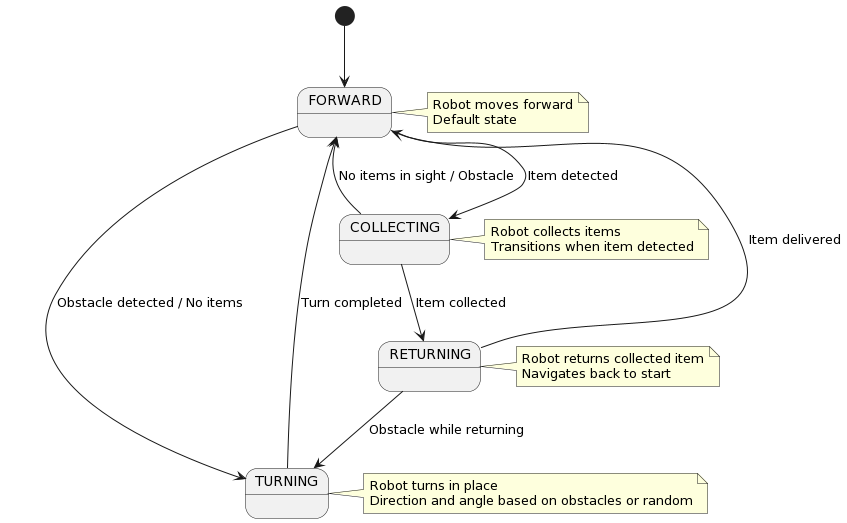
\includegraphics[width=\linewidth]{statediagram.png}}
\caption{State Machine Representing Autonomy}
\label{fig:statemachine}
\end{figure}

\subsection{Autonomy Realization}
% Discuss how autonomy is achieved, referencing Fig.~\ref{fig:statemachine}.
Autonomy in the system is achieved through a well-defined finite state machine (FSM), as depicted in Fig.~\ref{fig:statemachine}. The FSM has 4 states in which it can be: FORWARD, TURNING, COLLECTING, and RETURNING. It transitions based on sensor inputs and internal logic, also shown in Fig.~\ref{fig:statemachine}.

\subsection{Sensor Integration and Data Processing}
Integrating sensors like LiDAR and cameras is key to the robot's perception capabilities. Using ROS 2, sensor data is processed in real-time, with custom callback functions handling the data for tasks like obstacle detection and item identification. Without this processed information, navigation decisions and effective task execution would be impossible.

\subsection{Actuation and Movement Control}
Movement control within the system is made through the generation of Twist messages. Those messages determine the robot's linear and angular velocities, and are based on the current state of the FSM and the processed sensor data. This shows a direct link between sensory input and actuator output.

\subsection{Challenges and Solutions}
% Optionally, discuss any challenges faced during implementation and how you addressed them.
% Example: One challenge faced during implementation was ...
During the early phases of the development process, I started with designing and implementing a system for a single robot. This approach, however, later caused issues whilst integrating the multi-robot solution. One such issue was all robots transitioning to the RETURNING state once one of them collected an item. This was due to the lack of optimisation for a multi-robot system. For instance, the \texttt{item\_holder\_callback} method was returning all the bots' information simultaneously, which caused the issue. The solution was to ensure each robot received and acted upon only the information relevant to itself. This change made the system effectively manage the state transitions for each robot independently and further align with the demands of a multi-robot system.

% Add any additional subsections as necessary for your implementation details.

\section{Analysis}
\subsection{Experimental Approach}
%Describe your approach to experimental analysis.

%To evaluate the performance and efficiency of the system, I've taken a comprehensive experimental approach. The approaches were: logging data into the terminal, visually looking for problems while the simulations were running, and analyzing data logs from 10 different simulations (5 minutes each real time, 1:30 minutes roughly simulation time, different item distribution "seeds" were used in each simulation). Repeated trials were performed to ensure the reliability of the system.

%To evaluate the performance and efficiency of the system, I've taken a comprehensive experimental approach. This involved a multiple strategies to gather both qualitative and quantitative data. Firstly, extensive data logging into the terminal was performed to capture real-time operational details. Secondly, visual inspections were conducted during simulations to identify any immediate issues in the system's behavior. Finally, detailed analyses were carried out on data logs from 10 different simulations, each lasting 5 minutes in real-time (approximately 1:30 minutes in simulation time in my environment). These simulations were varied using different item distribution 'seeds' to test the system's robustness and adaptability under diverse conditions. Repeated trials ensured the reliability and consistency of the system’s performance across various scenarios.

To evaluate the performance and efficiency of the system, I've taken a comprehensive experimental approach. This involved multiple strategies to gather both qualitative and quantitative data:
\begin{itemize}
    \item \textbf{Data Logging}: Extensive data logging into the terminal was performed to capture real-time operational details of the system - This helped find bugs and solve issues.
    \item \textbf{Visual Inspections}: During simulations, visual inspections / Analysis were done to identify and fix issues in the system's behavior.
    \item \textbf{Simulation Analysis}: Detailed analysis of data logs from 10 different simulations, each lasting 5 minutes in real-time (approximately 1:30 minutes in simulation time in my environment). These simulations each used different item manager 'seeds' to assess the system's efficiency and adaptability under different conditions.
\end{itemize}
Repeated trials were also conducted to ensure the reliability and consistency of the system’s performance across various scenarios.


\subsection{Results}
% Present and interpret your results, both qualitative and quantitative.
The results of the experiments are presented in Fig.~\ref{fig:performancegraph} and Table~\ref{tab:performance}. 
%Qualitatively, the system demonstrated high levels of efficiency in navigating through the simulated environment and successfully retrieving items. Quantitatively, the performance metrics indicate ...

\begin{figure}[htbp]
\centerline{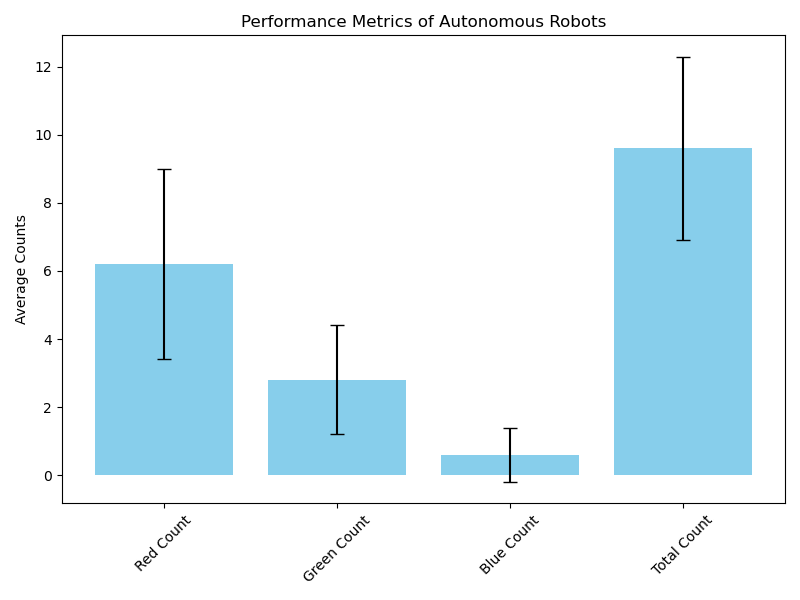
\includegraphics[width=\linewidth]{performance_metrics.png}}
\caption{Performance Analysis Graph}
\label{fig:performancegraph}
\end{figure}

\begin{table}[htbp]
\caption{Performance Metrics}
\begin{center}
\begin{tabular}{|c|c|c|}
\hline
Metric & Average & Standard Deviation \\
\hline
Red Count & 6.2 & 2.79 \\
Green Count & 2.8 & 1.60 \\
Blue Count & 0.6 & 0.80 \\
Total Count & 9.6 & 2.69 \\
\hline
\end{tabular}
\label{tab:performance}
\end{center}
\end{table}

\subsection{Results Analysis}
%Qualitatively, the system demonstrated decent results for collecting the items with a rounded average of 10 items per simulation. The red items were the most collected due to them being the closest to the home zone, green after due to them being mostly in the middle, and blue in last due to them being the furthest away. The robots are programmed to prioritise blue, then green then red items within its FOV when going to collect but this doesnt show in the results, let's see why.

%Quantitavely, this can be explained thanks to the visual inspections done during the simulations. Whilst the robots prioritise the blue items, they end up picking up green / red items on their way to getting the blue ones, thus transitioning to return state. Or if they reach the blue ones, they transition to returning state, they end up swapping the held item (in this scenario blue items) with other colored items (mostly reds cuz theyre the closest to the home) when they're driving back home. The items are swapped because thats how the item manager is made, unsure if its a bug or intentional. Could've treated the items as obstacles when robot is in return state (holding an item) but that would result in the robot taking too much time to return and would result in the total count average dropping quite a bit. but would result in more blue and green items overall.

Qualitatively, the system showed decent performance in item collection, with an average of approximately 10 items per simulation. Notably, red items were collected most frequently, as they were positioned closest to the home zone. Green items, typically located in the middle, were collected next in frequency, followed by blue items, which were the furthest away. Despite the robots being programmed to prioritize blue, then green, and then red items within their field of view (FOV) when collecting, this priority order was not reflected in the results.

Quantitatively, the reason behind this can be understood through visual inspections conducted during the simulations. While the robots initially prioritize blue items, they often collect green or red items en route to the blue ones, leading them to transition to the returning state prematurely. Additionally, on their way back to the home zone with a blue item, they frequently swap it for more readily accessible red items. This behavior is linked to the functionality of the item manager, though it is unclear whether this is a bug or an intentional design choice. An alternative approach could have been to treat untargeted items as obstacles when the robot is in the returning state, which would prevent item swapping. However, this could significantly increase the time taken for the robot to return home, potentially decreasing the total count of collected items but possibly resulting in a higher count of blue and green items.


\section{Evaluation}
Discuss the strengths and weaknesses of your solution based on your design, implementation, and analysis. Address the transferability of your solution from simulation to reality.

\section{Safety and Ethics}
Discuss safety implications and ethical considerations of autonomous robotic item retrieval in real-world scenarios. Reflect on how these relate to your solution.

\section{Conclusion}
Summarize your findings and suggest future work or improvements.

\bibliographystyle{IEEEtran}
\bibliography{references}

\end{document}
